\documentclass{standalone}
\usepackage{pgfplots}
\usepgfplotslibrary{groupplots}

\begin{document}
%\centering

\begin{tikzpicture}
  \pgfplotstableread{datafile.dat}\myscatter
  \begin{groupplot}[
      group style={
        group size=1 by 2,
        horizontal sep=0pt, vertical sep=0pt,
        xticklabels at=edge bottom,yticklabels at=edge left},
      height=6cm,width=6cm
    ]
\pgfmathsetmacro\a{2}
\pgfmathsetmacro\b{2}
\pgfmathsetmacro\c{\a+\b}

    \pgfplotsinvokeforeach{1,...,\c} {
    \nextgroupplot
    \pgfmathsetmacro\x{mod(#1-1,\a)}
    \pgfmathsetmacro\y{floor((#1-1)/\b)}

        \addplot+[only marks] 
          table[header=false,x index=\x,y index=\y]
          {\myscatter};
    }
  \end{groupplot}
\end{tikzpicture}

\begin{tikzpicture} 
  \pgfplotstableread{datafile.dat}\myscatter
  \begin{groupplot}[
      group style={
        group size=1 by 2,
        horizontal sep=0pt, vertical sep=0pt,
        xticklabels at=edge bottom,yticklabels at=edge left},
      height=6cm,width=6cm
    ]
\pgfmathsetmacro\a{2}
\pgfmathsetmacro\b{2}
\pgfmathsetmacro\c{\a+\b}

    \pgfplotsinvokeforeach{1,...,\c} {
    \nextgroupplot
    \pgfmathsetmacro\x{mod(#1-1,\a)}
    \pgfmathsetmacro\y{floor((#1-1)/\b)}


        \addplot+[only marks] 
          table[header=false,x index=\x,y index=\y]
          {\myscatter};
    }
  \end{groupplot}
\end{tikzpicture}

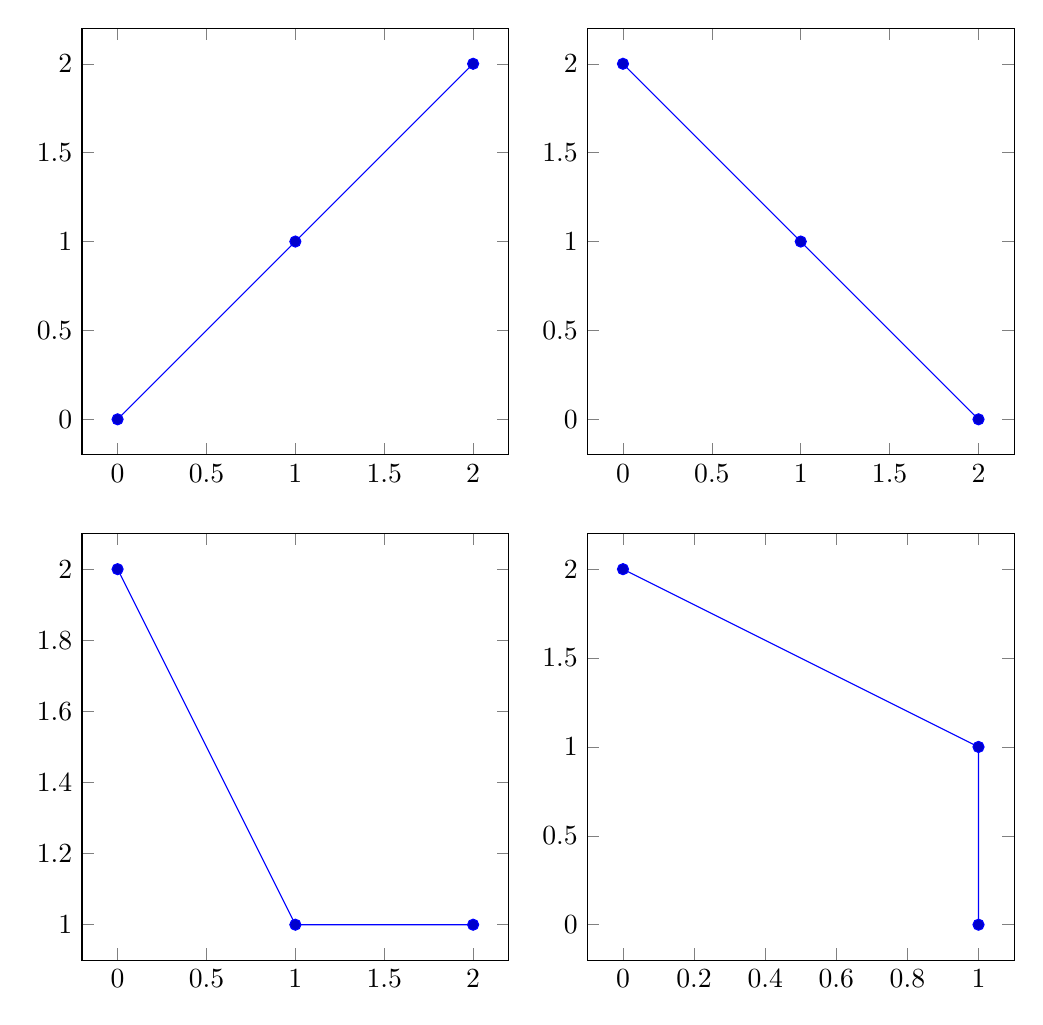
\begin{tikzpicture}
\begin{axis}[name=plot1,height=7cm,width=7cm]
\addplot coordinates {(0,0) (1,1) (2,2)};
\end{axis}
\begin{axis}[name=plot2,at={($(plot1.east)+(1cm,0)$)},anchor=west,height=7cm,width=7cm]
\addplot coordinates {(0,2) (1,1) (2,0)};
\end{axis}
\begin{axis}[name=plot3,at={($(plot1.south)-(0,1cm)$)},anchor=north,height=7cm,width=7cm]
\addplot coordinates {(0,2) (1,1) (2,1)};
\end{axis}
\begin{axis}[name=plot4,at={($(plot2.south)-(0,1cm)$)},anchor=north,height=7cm,width=7cm]
\addplot coordinates {(0,2) (1,1) (1,0)};
\end{axis}
\end{tikzpicture}
%\centering

\end{document}
